% This is samplepaper.tex, a sample chapter demonstrating the
% LLNCS macro package for Springer Computer Science proceedings;
% Version 2.20 of 2017/10/04
%
\documentclass[runningheads]{llncs}
%
\usepackage{graphicx}
% Used for displaying a sample figure. If possible, figure files should
% be included in EPS format.
%
% If you use the hyperref package, please uncomment the following line
% to display URLs in blue roman font according to Springer's eBook style:
% \renewcommand\UrlFont{\color{blue}\rmfamily}

\begin{document}
%
\title{Distributed population-based optimization for a fuzzy path tracking controller}
%
\titlerunning{Distributed population-based optimization}
% If the paper title is too long for the running head, you can set
% an abbreviated paper title here
%
\author{Mario García-Valdez\inst{1}\orcidID{0000-0002-2593-1114} \and
Alejandra Mancilla\inst{1}\orcidID{0000-0003-0430-8152} \and
Oscar Castillo\inst{1}\orcidID{0000-0002-7385-5689} \and 
Juan Julián Merelo-Guervós\inst{2}\orcidID{0000-0002-1385-9741}}
%
\authorrunning{García-Valdez et al.}
% First names are abbreviated in the running head.
% If there are more than two authors, 'et al.' is used.
%
\institute{Tijuana Institute of Technology / Tecnólogico Nacional de México, Tijuana, Baja Califorina,Calzada Tecnológico S/N, 22414, Mexico
\email{\{mario, alejandra.mancilla\}@tectijuana.edu.mx,ocastillo@tectijuana.mx} \and
Department of Computer Engineering, Robotics and Automation, University of Granada, Spain
\email{jmerelo@ugr.es}}
%
\maketitle              % typeset the header of the contribution
%
\begin{abstract}
  We propose a distributed bio-inspired algorithm that optimizes the parameters
  of a fuzzy controller, using a multi-population multi-algorithmic approach.
  The proposed algorithm can mix different metaheuristics, one for each
  population, with the aim of keeping the total population diversity high. To
  validate the speed-up benefit of our proposal, we optimized the membership
  functions of a fuzzy controller for tracking the trajectory of a mobile
  autonomous robot using populations running only Genetic Algorithms and
  Particle Swarm Optimization, and a mixed configuration where both algorithms
  run at the same time. Results indicate that even when we use random
  heterogeneous parameter configuration for the distributed populations, we
  obtain an error similar to other works while significantly reducing the
  execution time.  \textit{ This is a summary of our work ``Distributed and
    asynchronous population-based optimization applied to the optimal design of
    fuzzy controllers'' published in Symmetry in 2023. \cite{garcia2023}}
  \keywords{Fuzzy Control \and Bio-inspired Algorithms \and Distributed
    Algorithms.}
\end{abstract}
%
%
%
\section{Introduction}

Fuzzy logic control has been one of the most successful intelligent control
techniques \cite{Driankov2013Fuzzy},  one of its advantages being the use of a fuzzy
inference system (FIS) that creates a model with fuzzy rules as the
knowledge base. These rules have human interpretation but need to be
automatically or manually tuned, to handle the particularities of real-world
problems. In the case of FISs, the core components are the fuzzy propositions
constructing the fuzzy rules, these propositions are, in turn, constructed
using fuzzy variables and fuzzy terms that are defined using Membership Functions (MFs). Optimizing
the MFs parameters is challenging; as we need to execute one or more
simulations to establish the performance of just one configuration.

Our main contribution is to propose a distributed optimization method that
speeds up the tuning of fuzzy control optimization problems with respect to
sequential versions, without increasing the complexity for the user. This work
proposes a multi-population, distributed optimization method considering
current practices in constructing highly scalable, resilient, and replicable
systems. Moreover, the architecture is capable of executing several
bio-inspired algorithms simultaneously. We also address the problem of setting
the parameters for each population, this is an important factor in
multi-populations algorithms because it has been found in other works to have
an impact on the execution time and the optimization results. We compare two
strategies: the homogeneous setting using the same parameters in all
populations, and the other, a heterogeneous strategy using distinct parameters
for all populations.

\section{Proposed Method}

In this model, we have a  multi-population cycle in which a set of populations
$P$, each in a current state $j$, and a set ($W$) of $w$ workers, is added to a
message queue. Then each population ($population_{i}$) is pulled set of
populations by one of the workers. Then, after executing a metaheuristic, it
sends the evolved population ($X_{j+1}$) to the \emph{mixer}. The 
\emph{mixer} swaps some candidate solutions between two populations, changing
their state again and sending the resulting populations again to the input
message queue to be processed again by some worker, closing the cycle. Each
population has several parameters, including the algorithm to be executed on
that particular population, and the parameters of that metaheuristic. A single
population is executed several times during the lifetime of the algorithm, and
this number is limited by the parameter $nc$ (number of cycles).  A schematic
of an execution cycle is shown in Figure~\ref{fig:worker-pop}. A worker is an
agent running in a single process or thread. The worker pulls population
messages from a queue and executes the specified metaheuristic.

\begin{figure}
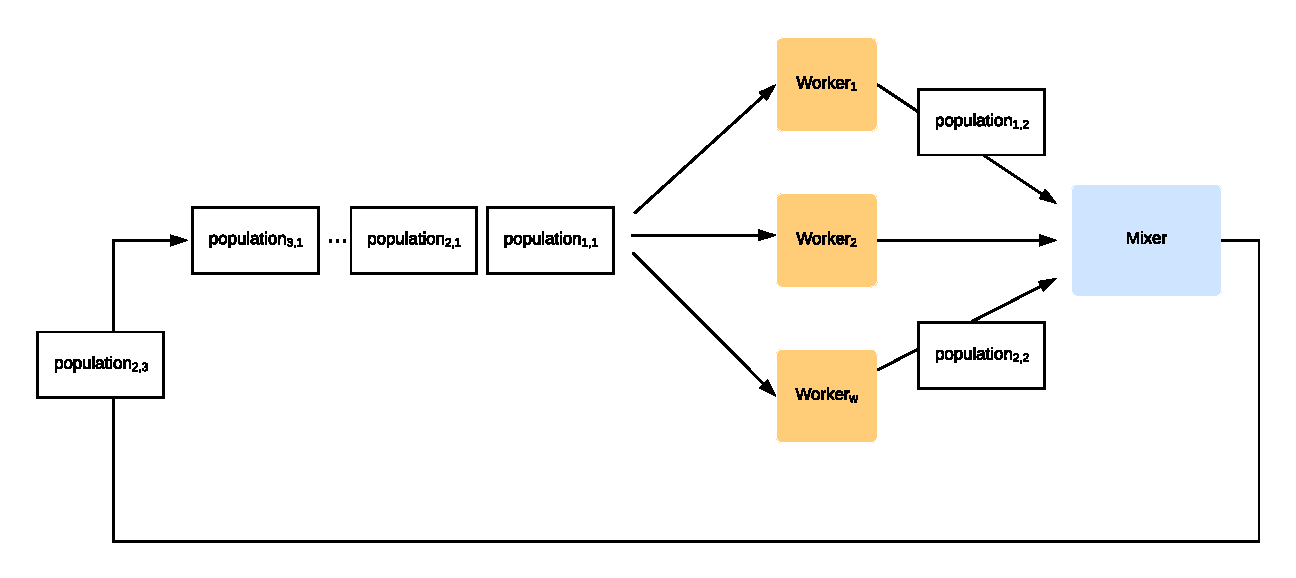
\includegraphics[width=\textwidth]{images/worker-pop}
\caption{ Our algorithm includes a set of populations $P$ in a current state $j$
  and a set of workers, which process ($population_{i}$) sending the evolved
  population to the \emph{mixer}, which swaps some candidate solutions between
  two populations, changing their state again and sending the resulting
  populations once more to be processed by workers, closing the cycle.
}\label{fig:worker-pop}
\end{figure}

\section{Experimental Results}

To validate the algorithm’s speed-up and optimization capabilities, we selected
the computationally demanding task of tuning a path-tracking fuzzy controller
for a bicycle-like mobile robot. The fuzzy controller we optimized in this work
has two input variables $\theta_e$ and $e$, indicating the angular error and
the distance  to the desired path. The controller has a single output $\omega$,
used for steering the front wheel. All three variables have the same
granularity using five fuzzy terms: \emph{high negative}, \emph{medium
negative}, \emph{low}, \emph{medium positive}, and \emph{high positive}. The
sign of the error indicates if the angle is to the left or right of the path.
We used 15 parameters for the MFs. To test each controller, they had to guide
the robot through three paths defined using cubic splines.
The average RMSE obtained from these simulations is the fitness of each 
controller. We selected the GA and PSO algorithms for the multi-population-based
algorithms, we selected the GA as lower-end algorithm specialized in combinatorial 
optimization and, on the other hand, the PSO algorithm which had the best results in
previous experiments. Furthermore, in previous works, but using
continuous optimization benchmarks, the combination of both metaheuristics
performed better than any of them alone.

When selecting the metaheuristics parameters, we also experimented with two
strategies, one establishing the same parameters for all populations, these
parameters are selected after running more than 30 trial experiments, we call
this a homogeneous parametrization. The other option is using a heterogeneous
strategy proposed by Gong et al. \cite{gong2011distributed} that randomly sets
the parameters of each population. For the GA, we used a tournament selection
with ($k=3$), a Gaussian mutation with $\mu = 0.0$ and $\sigma = 0.2$, and a
probability of $0.3$. We use a one-point crossover with a probability of $0.7$.
For the sequential PSO algorithm, we used a minimum and maximum speeds of
$-0.25$ and $0.25$, respectively, and $C_1=2$ and $C_2=2$. In the sequential
case, both algorithms have a single population of 50 candidate solutions and
run for 20 iterations. In the sequential version, the number of function
evaluations is 1000. This number is obtained by multiplying the population size
by the number of iterations. For the multi-population versions of the GA and
PSO algorithms. We used the same parameters as the sequential versions for the
homogeneous parametrization. We used the same parameters for the heterogeneous
versions as before, except for the following parameters affecting the
exploration-exploitation balance in the GA and PSO algorithms. The mutation
probability is selected for the GA from the $[0.1,0.5]$ range and the crossover
probability from $[0.3,0.9]$. For the PSO algorithm, we also selected the
minimum speed between $[-0.30,-0.20]$ and the maximum from $[0.20,0.30]$. Both
$C_1$ and $C_2$ are in the $[1.0,2.0]$ range. For all the distributed versions,
we set the number of populations (islands) to seven, each with a population
size of nine. Each worker will execute four iterations (generations) of the
algorithm. All populations will complete four cycles; this means they will pass
through the mixer module four times. As a result, the total number of function
evaluations is 1008. About % ? same order of magnitude? Exact same number? - JJ
% same number, it was mentioned at few sentences back. - M
the same as the sequential, single-population 
versions (1000 iterations). The results are shown in Table~\ref{tab:speedup}.


\begin{table}[]
\caption{
  Time to solution in 30 observations for each of the
    presented algorithms. The execution time is expressed in seconds.
    }\label{tab:speedup}
\renewcommand*{\arraystretch}{1.4}
\setlength{\tabcolsep}{5pt}
    \begin{small}
\begin{tabular}{lrrrrrrrr}
    \hline
				&  \multicolumn{2}{c}{Sequential} & \multicolumn{6}{c}{Distributed} \\
    \hline
    & &    & \multicolumn{3}{c}{Homogeneous} & \multicolumn{3}{c}{Heterogeneous} \\
    \cline{4-6} \cline{7-9}
       & \multicolumn{1}{c}{GA} & \multicolumn{1}{c}{PSO} &\multicolumn{1}{c}{GA} & \multicolumn{1}{c}{PSO} & \multicolumn{1}{c}{PSO-GA} &\multicolumn{1}{c}{GA} & \multicolumn{1}{c}{PSO} & \multicolumn{1}{c}{PSO-GA}\\
    \hline
    Speed-up & \multicolumn{1}{c}{-} & \multicolumn{1}{c}{-} & 4.74 & 6.86 & 6.60 & 5.05 & 6.84 & \underline{6.95} \\
    \hline
Avg.   & 1999.34 & 2851.61 & 421.67 & 415.64 & 431.52 & 395.75 & 415.79 & 409.90 \\
    \hline
STDs.   & 82.44   & 278.73  & 28.54           & 23.47                    & 22.60           & 26.54           & 20.47           & 24.85    \\
    \hline
Min    & 1876.40 & 2457.98 & 364.65          & 365.81                   & 394.61          & 340.65          & 374.83          & 372.20   \\
    \hline
Max    & 2253.71 & 3822.01 & 526.76          & 467.47                   & 478.80          & 461.46          & 461.96          & 465.27  \\
    \hline
\end{tabular}
    \end{small}
\end{table}

\section{Concluding Remarks}

These results confirm that a multi-population-based strategy offers a convenient
speed-up compared with the sequential versions with no loss of algorithmic
performance.  Moreover, combining the continuous optimization capabilities of a
PSO algorithm with the faster GA metaheuristic offers better execution times
than the single algorithm alternatives.  Finally, the heterogeneous strategy
that used randomized configuration parameters gave better execution times when
using the PSO-GA variant.

%
% the environments 'definition', 'lemma', 'proposition', 'corollary',
% 'remark', and 'example' are defined in the LLNCS documentclass as well.
%
% ---- Bibliography ----
%
% BibTeX users should specify bibliography style 'splncs04'.
% References will then be sorted and formatted in the correct style.
%
\bibliographystyle{splncs04}
\bibliography{symmetry}
%
\end{document}
